\documentclass[colorback,accentcolor=tud1c,11pt]{tudreport}
\usepackage[english]{babel}
\usepackage[utf8x]{inputenc}
%\usepackage[T1]{fontenc}

%\usepackage[stable]{footmisc}
%\usepackage[ngerman,pdfview=FitH,pdfstartview=FitV]{hyperref}

\usepackage{booktabs}
%\usepackage{multirow}
%\usepackage{longtable}
\usepackage{listings}
\usepackage{graphicx}
\usepackage{subfigure} 	
\usepackage{float}
\usepackage{amsmath}
\usepackage{hyperref}

\newcommand\todo[1]{\textcolor{red}{#1}}
\newcommand\code[1]{\texttt{#1}}
%\usepackage{floatflt}

\graphicspath{{./img/}}

%\newlength{\longtablewidth}
%\setlength{\longtablewidth}{0.675\linewidth}

\title{Mini-task report: FlowMap Lut-Packing Algorithm}
\subtitle{Ludwig Meysel, Mitja Stachowiak}

\begin{document}
\maketitle



\chapter{Introduction}
The task was to implement a simple version of the Flow Map algorithm which is used to bring arbitrary boolean functions and - networks to PCBs with limited size of lookup tables.


\chapter{BLIF Parser}
The Parser of the Espresso-project is used again and developed further; especially the functions are now stored in a graph-structure. It is still ready-to-use for the Espresso-package. The parser now also supports latches and sub-circuits in a basically way that enables it to hold this information in memory and save it back to file.

\chapter{Labelling}
The labelling phase is more or less the heart of the FlowMap algorithm. What happens here, is the first step to build clusters which later will be stored into LUTs. For this part, the graph is assumed to be already decomposed so that each node (gate) has maximum two inputs for the highest granularity of the graph. That means for LUT packing there is a maximum flexibility for each node to pack it into the predecessor or successor LUT.

\section{Excursus: The used Ford-Fulkerson implementation and its graph model}
The used implementation of Ford-Fulkerson is part of a library called \textit{algs4} published by the department of computer science of the princeton university.
\par
How Ford-Fulkerson actually works is not part of this report. Essentially it finds the maximum flow in a directed graph. "Maximum flow" may be imagined as a value giving information about a volume-unit passing through pipes, whereas the graph edges representing those pipes. The whole graph is then a network of pipes. Having one pipe at the end of the net with a certain diameter (edge weight), it will be the bottleneck of the whole net. The whole net cannot handle a higher flow than the last pipe. What Ford-Fulkerson does, is to find this maximum. Furthermore this implementation gives information about which edges limit the flow, which will be necessary later because there is the \textit{min-cut}.
\par
The graph model is pretty simple: It just consists of a number saying how many nodes are contained in the graph. The edges are pairs of two numbers, the target and destination node (respectively their indices). A graph with two nodes $A$ and $B$ and an edge $A\rightarrow B$ would be described in Java as a Graph having two nodes and an Edge \{0,1,\textit{weight}\}.
\par
This graph model is not suitable for many purposes (e.g. decomposition) because it is not really object oriented. But due to its simplicity it is very comfortable to use for the Ford-Fulkerson part within FlowMap because FlowMap must create one derived graph for Ford-Fulkerson for each node of the original decomposed graph. Therefore the lightweight model is very convinient for this purpose.
\par
Finally, to run Ford-Fulkerson the required parts of the original graph are brought to the simple model and after running Ford-Fulkerson the labels can be set (via a temporary mapping) back in the original graph.

\section{Node selection}
Having the decomposed graph, each \textit{primary input} (PI) is initially labelled with 0. Primary inputs are not packed into LUTs, therefore it is not necessary to run Ford-Fulkerson with only having the inputs \textit{selected}. In this context "selected" means the set of nodes which is given to Ford-Fulkerson, whereas the source-node is not a real node, but the target node is the currently examined node.
\par
For the labelling phase the nodes are ordered by their hierarchical height (i.e. node-height is $\max($predecessors-height$)+1$). By this ordering it is made sure, that all parent nodes have been labelled before the sucessors are going to labelled. When traversing this ordered list, Ford-Fulkerson must run for each node, whereas the \textit{current} node represents the target node. The graph, Ford-Fulkerson requires, needs not only a virtual source node added, but also each original node to be split up into two nodes having one edge to be connected (as described in the lecture \cite{Hochberger2017}). Furthermore, the currently examined node must contain each node of the current label-value. Using an object oriented graph model would not be a very good idea, because it would require a clone of nearly the whole graph, then do the transformations to run Ford-Fulkerson.
\par
Here is the simplified graph model of the algs4-library more suitable to do all subgraph-creation with the required transformations in just one step. The simple model is split up into four parts: original nodes, cloned nodes as well as source and target node. To create the graph the number of nodes is required. Therefore Graph must be traversed from the current node upwards to the PIs. Each node with a smaller label than the currently examined label-value is an explicit node in the simplified model. Having $n$ nodes to transfer into the temporary graph, then it has $|V|=2*n+2$ nodes in total. $2*n$ for the nodes to be split up, as well as source and target. When the test for the target node is e.g. whether it has label 3 or 4, then all label-3-nodes are collapsed into the target node. That means the label-3-nodes are just not added to the graph but the edges going \textbf{to} an label-3-node are added to the target node. The PIs are just predecessors of the virtual source.
\par
The splitting is also done by just adding the edges correctly: In $|V|$ the first $n$ indices represent the original nodes, the second $n$ nodes are their split-nodes. For each node the predecessor's (original) index is then just adding $n$.
\begin{table}[]
	\centering
	\begin{tabular}{|cccccc|cccccc|cc|}
		\hline
	A & B & ... & G & H & I & A' & B' & ... & G'  & H'  & I'  & s  & t  \\
		\hline
	0 & 1 &  ... & 6 & 7 & 8 & 9  & 10 & ... & 15 & 16 & 17 & 18 & 19 \\
		\hline
	\end{tabular}
	\caption{Alignment of the nodes in the simplified graph model}
	\label{tbl:simple-graph-model}
\end{table}
\begin{figure}
	\centering
	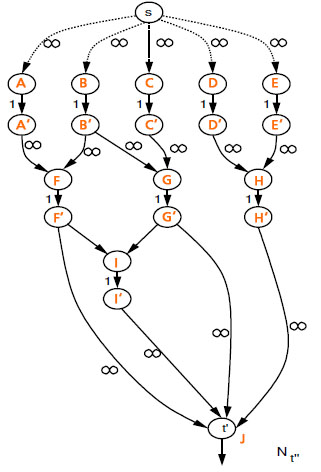
\includegraphics[width=.4\textwidth]{graph}
	\caption{A graph after transformation ready to run Ford-Fulkerson (Source: Modified from \cite{Hochberger2017})}
	\label{fig:split-graph}
\end{figure}

Table~\ref{tbl:simple-graph-model} depicts the alignment in the simplified graph model of the graph as in fig.~\ref{fig:split-graph}. In this example $n=9$, so the original nodes are represented with indices $0$ to $8$, the "clones" are $i+n$ with $i=0..8$. Source and target are the last two nodes. Now when adding the nodes A to I they can be split up by adding an Edge \{$i$,$i+n$\} with weight=$1$. The original edges are added with weight=$\infty$ - the predecessor indices must always be in the range of $[n,2n]$.

\section{Labelling the graph}
In fig.~\ref{fig:split-graph} the graph shall be labelled 5-feasability (i.e. this graph will be packed into 5-input-LUTs). When running Ford-Fulkerson on this graph, the min cut with max-flow of 5 will exist. Therefore the label has the same value like the node's predecessors. If there were no 5-feasable cut in the graph, the label-value would have been incremented.

\section{Getting the LUTs}
As already said, the Ford-Fulkerson implementation also gives information about \textit{where} the cut is, i.e. which edges limiting the max-flow. It makes sense, to store the destinations of each cut-edge in a \code{HashMap} which depicts the current node to the cut-edge's destination-nodes, because those will become the outputs of the preceding LUTs and therefore also the inputs of the LUT possibly created from the current node.
\par
When fig.~\ref{fig:split-graph} should be packed into 3-LUTs a min-cut would exist after nodes $F$, $G$ and $H$. When this would be the whole graph to pack, then the LUT of node $J$ had three preceding LUTs which is $F$, $G$ and $H$. Therefore for each node the min-cut-nodes are stored \textbf{if the min-cut is k-feasable}. If not, the immediate predecessors of a node are stored. Due to the decomposition, there are only two predecessors then.
\par
Now there are clusters built and the LUT packing can begin. Starting with the primary outputs (POs) a lookup in the cluster gives the input-nodes of the LUT. The nodes used as LUT inputs are also the outputs of another LUT and therefore they are the next key in the cluster, and so on. After creating all LUTs the LUT's boolean function must be composed from the related nodes.



\chapter{Conclusion}
Niemand interessiert die Conclusion   :P
\\
The project is realized in about ???? lines of code.



\bibliographystyle{plain}
\bibliography{references}

\end{document}

